\documentclass{assignment}
\ProjectInfos{研究型物理实验}{PHYS1703}{2020-2021学年第一学期}{Lab-2-Note-1-蔡氏电路简析}{2020. 10. 14(周三)}{陈稼霖}{45875852}
\begin{document}
\section*{要求}
\begin{itemize}
    \item 分析蔡氏电路中蔡氏二极管的$I-V$特性;
    \item 模拟以蔡氏电路中两电容两端电压为坐标的李萨如图.
\end{itemize}

蔡氏电路(Chua's circuit)是蔡少棠于1983年提出的一种非线性电路. 如图\ref{Chua's-circuit}所示,蔡氏电路是由一个电感$L$、两个电容$C_1$、$C_2$和一个蔡氏二极管$N_{\text{R}}$并联再串联一线性电阻$R$而成的LRC电路,其中蔡氏二极管为一有源非线性电阻,它的存在使得整个电路为一非线性系统,并使得两个电容两端电压的振荡呈现出混沌效应,对初始条件和外界扰动极为敏感. 下面我们首先分析蔡氏二极管的$I-V$特性,然后根据这一特性模拟在不同初始条件下电路的演化,并从两个电容器两端电压振荡的李萨如图中管窥混沌现象.

\begin{figure}[h]
    \centering
    \includegraphics[width=.5\columnwidth]{Chua'sCircuit.png}
    \caption{蔡氏电路}
    \label{Chua's-circuit}
\end{figure}

\section{蔡氏二极管的$I-V$特性}
蔡氏二极管(Chua's diode)可以用一些简单的电子元件搭建,而且实现方式多种多样. 本实验所用的蔡氏二极管由两个负阻抗转换器串联而成. 因此,我们先分析负阻抗转换器的$I-V$特性,然后由此得出蔡氏二极管的$I-V$特性.

\subsection{负阻抗转换器}
如图\ref{Chua's-diode}所示,负阻抗变换器(Negative impedance converter)是一个运算放大器上同时加了正反馈和负反馈得到.

\begin{figure}[h]
    \centering
    \includegraphics[width=.5\columnwidth]{Chua'sDiode.png}
    \caption{蔡氏二极管}
    \label{Chua's-diode}
\end{figure}

运算放大器(Operational amplifier,简称运放)具有5个端口,分别是反向端(即图\ref{NIC}中-号端)、非反向端(即图\ref{NIC}中+号端)、输出端(即图\ref{NIC}中三角形右边顶点端)、正电源端(即图\ref{NIC}中$V_{\text{pp}}$对应端口)和负电源端(即图\ref{NIC}中$V_{\text{nn}}$对应端口),其基本特性是可以在输出端产生正比于非反向端电压$V_+$和反向端(即图\ref{NIC}中-号端)电压$V_-$之差的电压
\begin{align}
    V_o=A\cdot(V_+-V_-),
\end{align}
其中系数$A$称开环差动增益,它的值极大,通常可达$10^6$. 当连接了运放的输出端和反向端,由于开环差动增益极大,当反向端电压稍低(高)于非反向端,则输出端电压急剧升高(降低),从而带动反向端电压升高(降低),形成负反馈,因此此时反向端和非反向端电压几乎相等,可近似视为短路(运放的虚短性质). 而由于运放输入阻抗很大,因此反向端和非反向端几乎无电流流入或流出运放,可以近似视为断路(运放的虚断性质).

\begin{figure}[h]
    \centering
    \includegraphics[width=.5\columnwidth]{NegativeImpedanceConverter.png}
    \caption{负阻抗变换器}
    \label{NIC}
\end{figure}

在图\ref{NIC}所示的负阻抗变换器中,由于运放的虚断,电流$I$几乎全部由负阻抗变换器+端经过$R_f$,而几乎没有经过运放,因此对$R_f$用欧姆定律有
\begin{align}
    \label{Rf-Ohm}
    I=\frac{V-V_o}{R_f}.
\end{align}
而根据$R_a$和$R_b$的分压,非反向端电压和输出端电压有如下关系:
\begin{align}
    V_n=\frac{R_b}{R_a+R_b}V_o.
\end{align}
又由于运放的虚短,
\begin{align}
    V=V_p=V_n.
\end{align}
上面三式联立可得,在运放的输出电压未达到饱和的条件下,负阻抗变换器$I-V$关系可表为
\begin{align}
    I=-\frac{R_a}{R_bR_f}V.
\end{align}
当运放的输出电压达到饱和,以正饱和为例,此时
\begin{align}
    V_o=&V_{\text{pp}}\\
    V=&\frac{R_b}{R_a+R_b}V_{\text{pp}},\\
    I=&-\frac{R_a}{R_f(R_a+R_b)}V_{\text{pp}}.
\end{align}
若继续增大负阻抗变换器两端的输入电压,则$V=V_p>V_n$,但运放输出电压不再增大,依然为$V_o=V_{\text{pp}}$,式\eqref{Rf-Ohm}依然成立,故负阻抗变换器此时的$I-V$关系可表为
\begin{align}
    I=\frac{V-V_{\text{pp}}}{R_f}.
\end{align}
同理可得当输入反向电流,使电压达到饱和后,负阻抗变换器的$V-I$关系变为
\begin{align}
    I=\frac{V-V_{\text{nn}}}{R_f}.
\end{align}
% 当运放的输出电压达到饱和,以负饱和为例,此时
% \begin{align}
%     V_o=&V_{\text{nn}}\\
%     V=&\frac{R_b}{R_a+R_b}V_{\text{nn}},\\
%     I=&-\frac{R_a}{R_f(R_a+R_b)}V_{\text{nn}}.
% \end{align}
% 若继续增大电流,则$V=V_p>V_n$,但输出电压(的绝对值)不再增大,依然为$V_o=V_{\text{nn}}$,式\eqref{Rf-Ohm}依然成立,故负阻抗变换器此时的$V-I$关系可表为
% \begin{align}
%     V=R_fI+V_{\text{nn}}.
% \end{align}
% 同理可得当输入反向电流,使电压达到饱和后,负阻抗变换器的$V-I$关系变为
% \begin{align}
%     V=R_fI+V_{\text{pp}}.
% \end{align}
综上,负阻抗变换器的$V-I$关系是非线性的:
\begin{align}
    I=\left\{\begin{array}{ll}
        \frac{V-V_{\text{nn}}}{R_f},&V<\frac{R_b}{R_a+R_b}V_{\text{nn}},\\
        -\frac{R_a}{R_bR_f}V,&\frac{R_b}{R_a+R_b}V_{\text{nn}}\leq V\leq\frac{R_b}{R_a+R_b}V_{\text{pp}},\\
        \frac{V-V_{\text{pp}}}{R_f},&V>\frac{R_b}{R_a+R_b}V_{\text{pp}}.
    \end{array}\right.
\end{align}
本实验中蔡氏二极管中的两个负阻抗变换器的$V-I$特性可分别表为
\begin{align}
    \notag I=f_1(V)=&H\left(-\frac{R_3}{R_2+R_3}V_1-V\right)\times\left(\frac{V+V_2}{R_1}\right)+H\left(\frac{R_3}{R_2+R_3}V_2-V\right)\times H\left(V+\frac{R_3}{R_2+R_3}V_1\right)\times\left(-\frac{R_2}{R_3R_1}V\right)\\
    \qquad&+H(V-\frac{R_3}{R_2+R_3}V_2)\times\left(\frac{V-V_1}{R_1}\right),\qquad(\text{负阻抗变换器1(含$R_1$,$R_2$,$R_3$)})\\
    \notag I=f_2(V)=&H\left(-\frac{R_6}{R_5+R_6}V_1-V\right)\times\left(\frac{V+V_5}{R_4}\right)+H\left(\frac{R_6}{R_5+R_6}V_2-V\right)\times H\left(V+\frac{R_6}{R_5+R_6}V_1\right)\times\left(-\frac{R_5}{R_6R_4}V\right)\\
    \qquad&+H(V-\frac{R_6}{R_5+R_6}V_2)\times\left(\frac{V-V_1}{R_4}\right),\qquad(\text{负阻抗变换器2(含$R_4$,$R_5$,$R_6$)})
\end{align}
其中用了单位阶跃函数$H(x)=\left\{\begin{array}{ll}
    0,&x<0\\
    1,&x>0
\end{array}\right.$来刻画$V-I$特性的分段性质,以方便在代码中的表示. 两个负阻抗变换器的$V-I$特性曲线分别如图\ref{NIC-I-V}所示.

\begin{figure}[h]
    \centering
    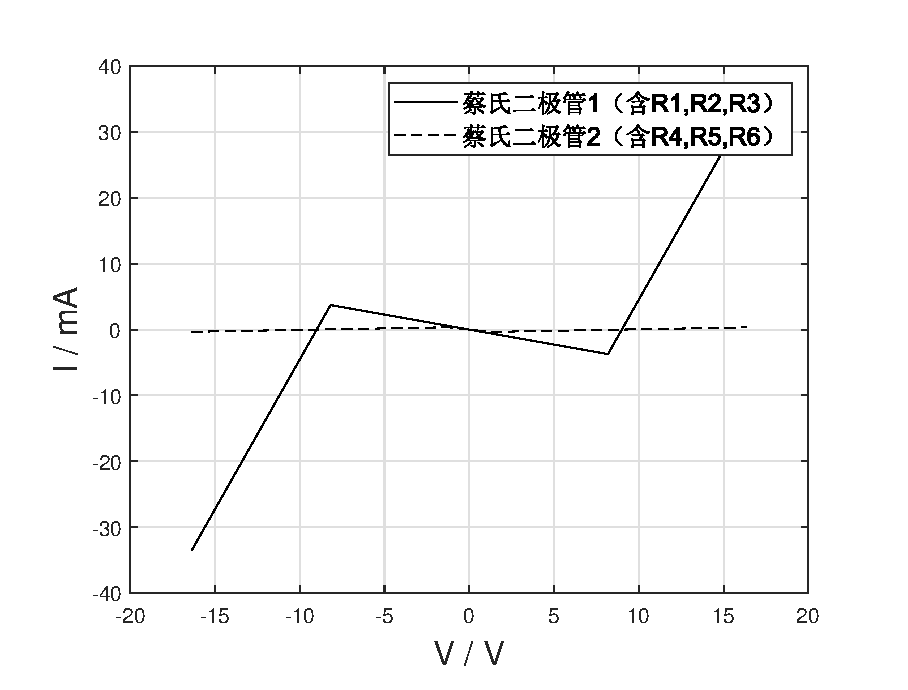
\includegraphics[width=.5\columnwidth]{NegativeImpedanceConverter-I-V.eps}
    \caption{负阻抗变换器$I-V$特性曲线}
    \label{NIC-I-V}
\end{figure}

\subsection{蔡氏二极管的$I-V$特性}
蔡氏二极管中两个负阻抗变换器并联,因此其总电压相等,总电流相加. 故蔡氏二极管的$I-V$特性为
\begin{align}
    I=f(V)=f_1(V)+f_2(V),
\end{align}
如图\ref{Chua's-diode-I-V}所示.

\begin{figure}[h]
    \centering
    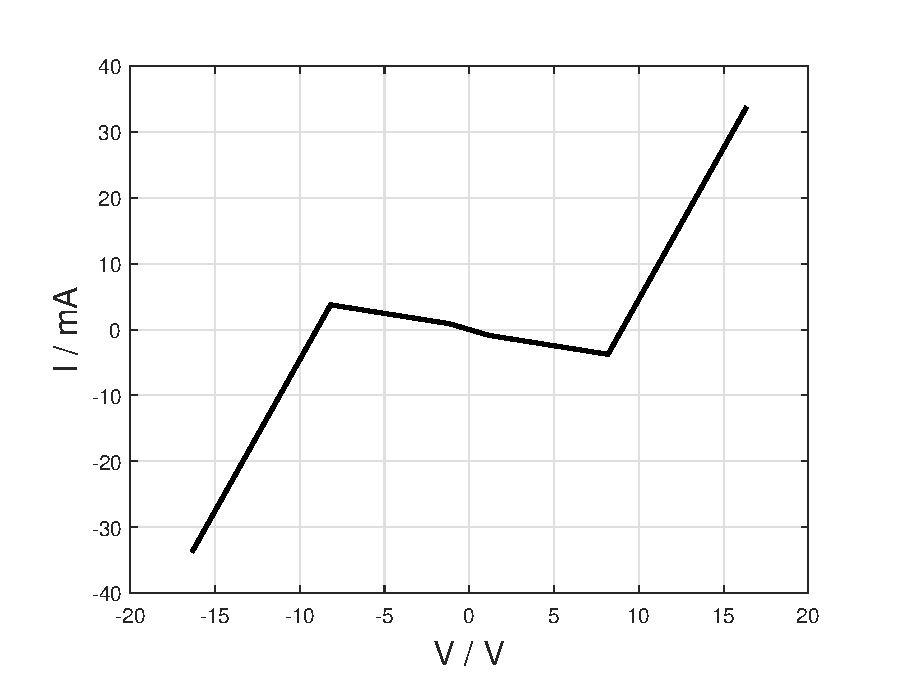
\includegraphics[width=.5\columnwidth]{ChuasDiode-I-V.eps}
    \caption{蔡氏二极管$I-V$特性曲线}
    \label{Chua's-diode-I-V}
\end{figure}

\section{蔡氏电路模拟}
蔡氏电路中,电感$L$两端的电压$V_{C2}$正比于通过电感的电流$I_L$的变化速率
\begin{align}
    \label{L}
    V_{C2}=-L\frac{\mathrm{d}I_L}{\mathrm{d}t}.
\end{align}
通过电容$C_2$的电流$I_{C2}$正比于电容$C_2$两端的电压$V_{C2}$的变化速率
\begin{align}
    \label{C2}
    I_{C2}=-C_2\frac{\mathrm{d}V_{C2}}{\mathrm{d}t}.
\end{align}
通过电容$C_1$的电流$I_{C1}$正比于电容$C_1$两端的电压$V_{C1}$的变化速率
\begin{align}
    \label{C1}
    I_{C1}=-C_1\frac{\mathrm{d}V_{C1}}{\mathrm{d}t}.
\end{align}
由基尔霍夫第二定律,从接地点开始经电容$C_2$、过可变电阻$R$和电容$C_1$回到接地点,电势变化为$0$:
\begin{align}
    V_{C2}-(I_L+I_{C2})R-V_{C1}=0.
\end{align}
故可将经过电容$C_2$的电流$I_{C2}$表为
\begin{align}
    \label{IC2}
    I_{C2}=\frac{V_{C2}-V_{C1}}{R}-I_L.
\end{align}
又由蔡氏二极管的$V-I$曲线有
\begin{align}
    I_N=f(V_{C1})
\end{align}
其中,根据基尔霍夫第一定律,经过蔡氏二极管的电流$I_N$可表为
\begin{align}
    I_N=I_L+I_{C1}+I_{C2}.
\end{align}
联立上面两式并代入\eqref{IC2}可将经过电容$C_1$的电流$I_{C1}$表为
\begin{align}
    \label{IC1}
    I_{C1}=f(V_{C1})-\frac{V_{C2}-V_{C1}}{R}.
\end{align}
将$I_{C1}$和$I_{C2}$的表达式\eqref{IC1}\eqref{IC2}分别回代入式\eqref{C1}\eqref{C2}并与式\eqref{L}联立得到微分方程组
\begin{align}
    \left\{\begin{array}{l}
        \frac{\mathrm{d}I_L}{\mathrm{d}t}=-\frac{1}{L}V_{C2},\\
        \frac{\mathrm{d}V_{C1}}{\mathrm{d}t}=-\frac{1}{C_1}\left[f(V_{C1})-\frac{V_{C2}-V_{C1}}{R}\right],\\
        \frac{\mathrm{d}V_{C2}}{\mathrm{d}t}=-\frac{1}{C_2}\left(\frac{V_{C2}-V_{C1}}{R}-I_L\right).
    \end{array}\right.
\end{align}

在不同的条件(改变可变电阻阻值$R$,改变初始条件$V_{C2}(t=0)$等)下求解以上微分方程组,得到蔡氏电路的$V_{C1}$和$V_{C2}$的演化轨迹如组图\ref{vary-R}和\ref{vary-VC2}所示.

\begin{figure}[h]
    \centering
    \subfigure[$R=1538\mathrm{\Omega}$]{
        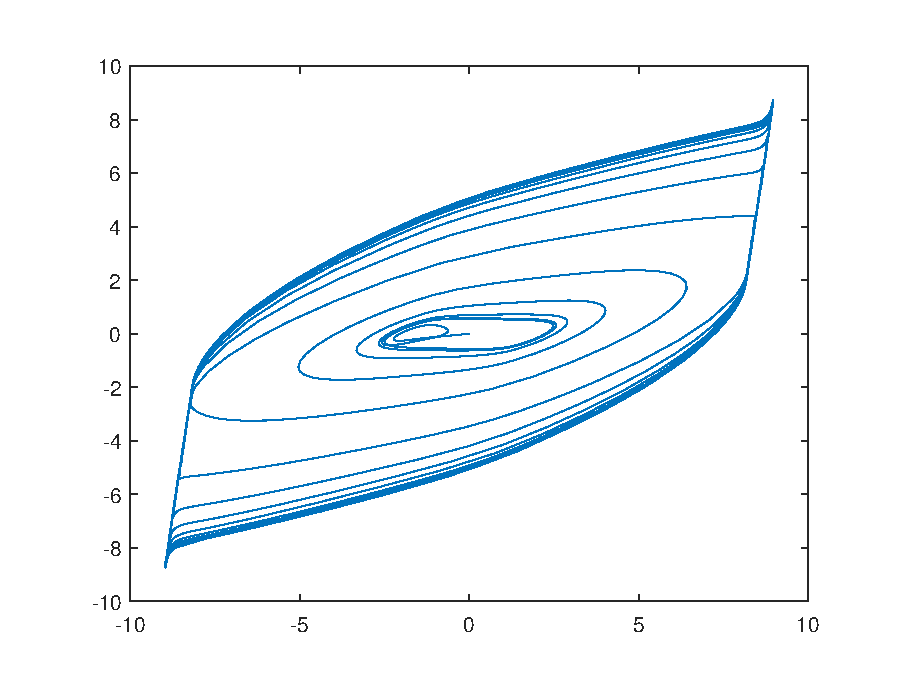
\includegraphics[width=.3\columnwidth]{R=1538,IL=0,VC2=0.01,VC2=-0.01.eps}
    }
    \subfigure[$R=1539\mathrm{\Omega}$]{
        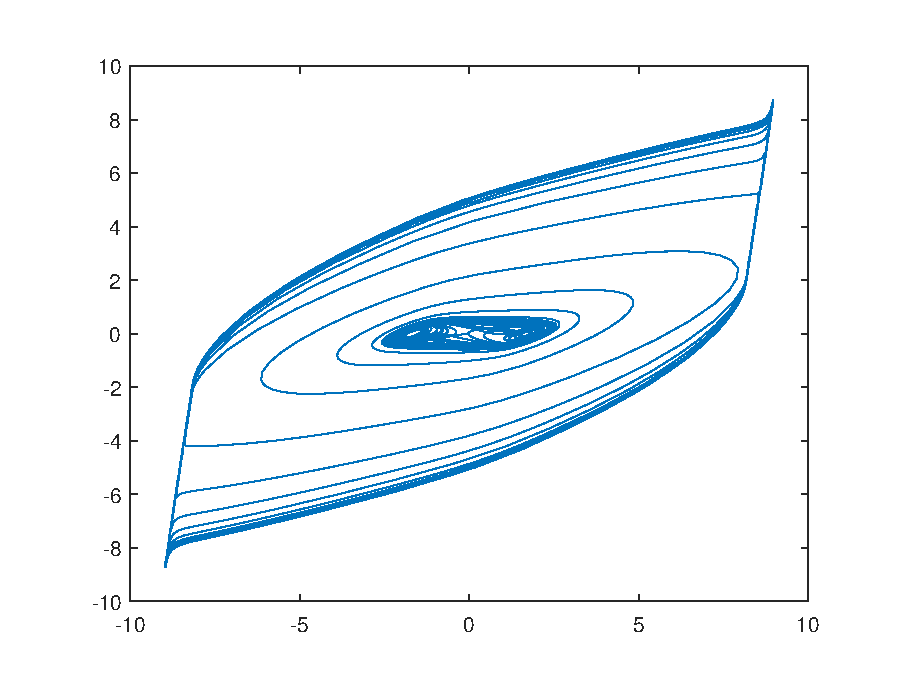
\includegraphics[width=.3\columnwidth]{R=1539,IL=0,VC2=0.01,VC2=-0.01.eps}
    }
    \subfigure[$R=1540\mathrm{\Omega}$]{
        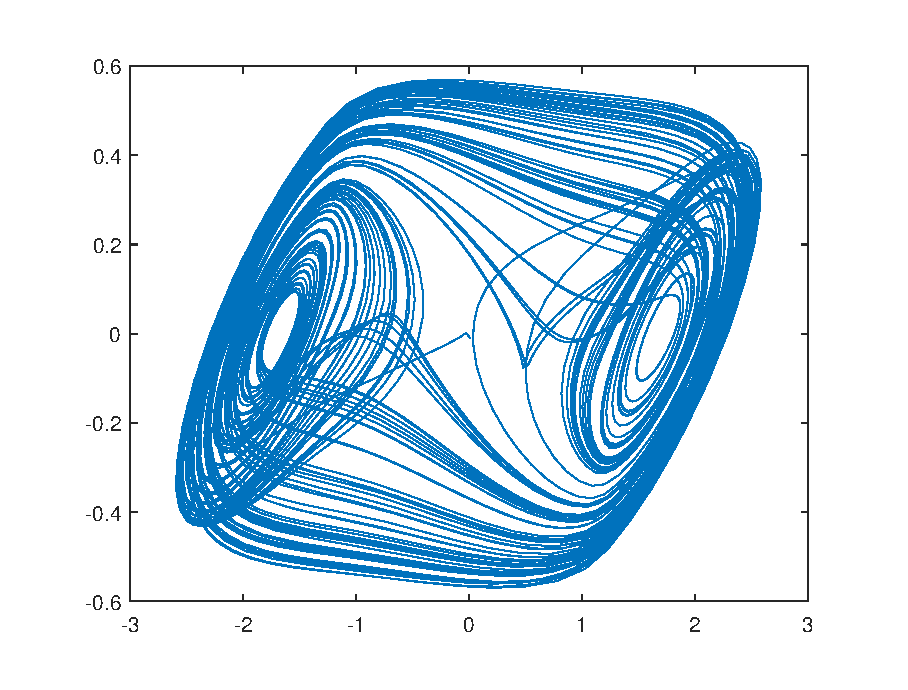
\includegraphics[width=.3\columnwidth]{R=1540,IL=0,VC2=0.01,VC2=-0.01.eps}
    }
    \subfigure[$R=1541\mathrm{\Omega}$]{
        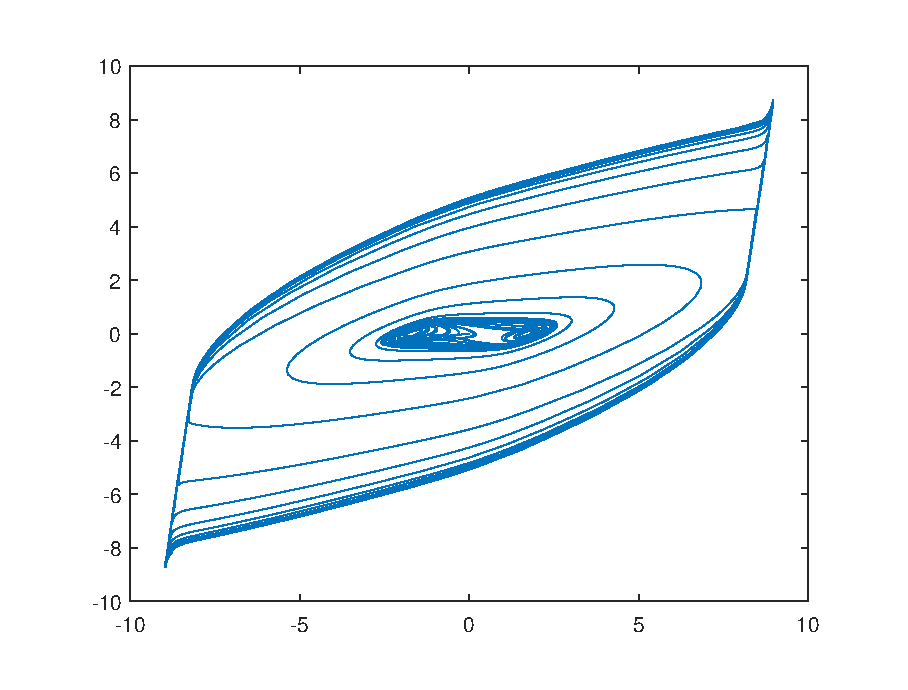
\includegraphics[width=.3\columnwidth]{R=1541,IL=0,VC2=0.01,VC2=-0.01.eps}
    }
    \subfigure[$R=1542\mathrm{\Omega}$]{
        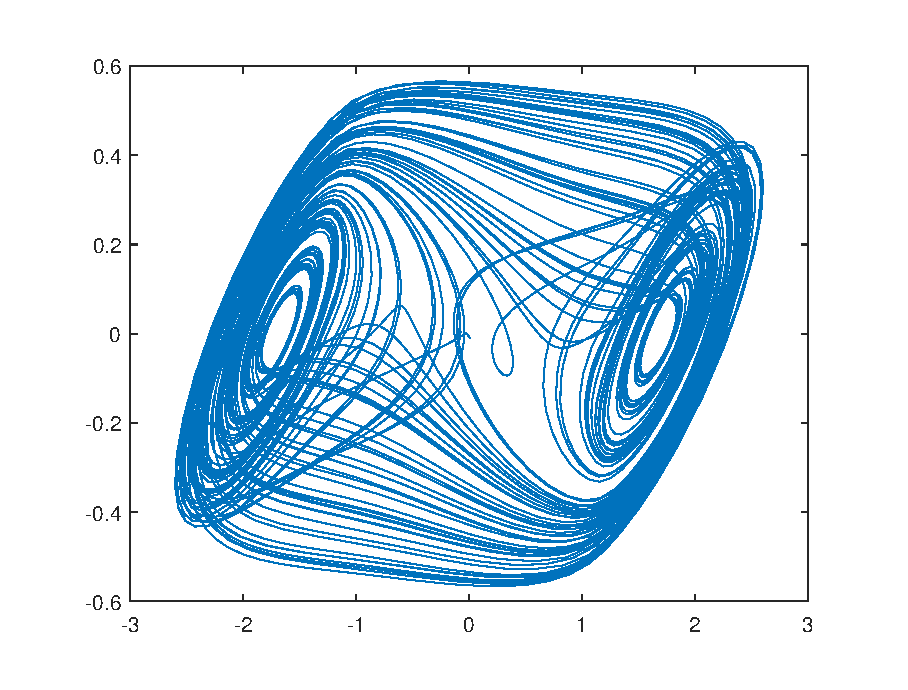
\includegraphics[width=.3\columnwidth]{R=1542,IL=0,VC2=0.01,VC2=-0.01.eps}
    }
    \subfigure[$R=1543\mathrm{\Omega}$]{
        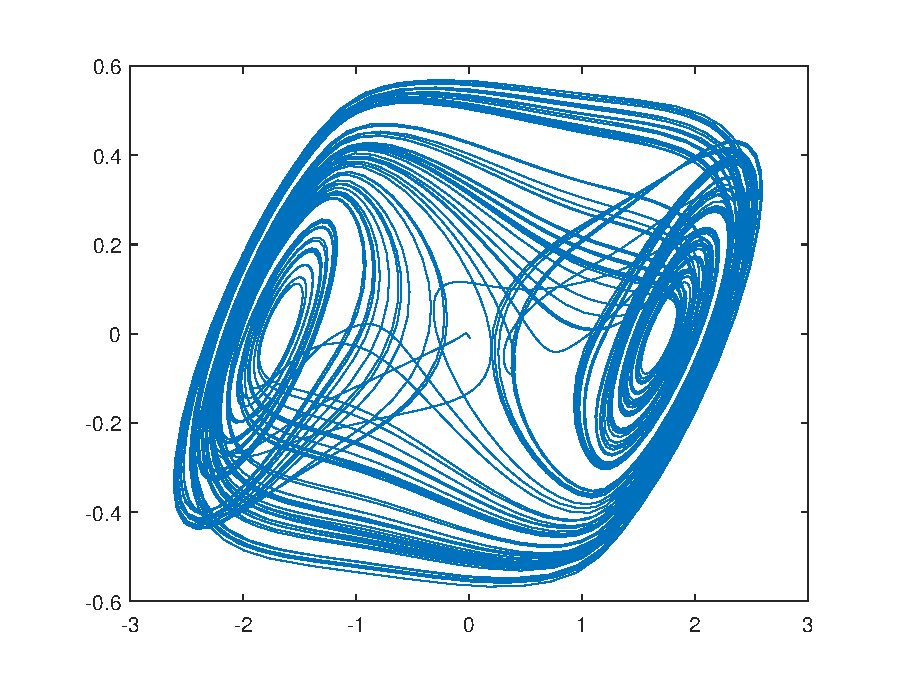
\includegraphics[width=.3\columnwidth]{R=1543,IL=0,VC2=0.01,VC2=-0.01.eps}
    }
    \caption{设定初始条件$I_L(t=0)=0$,$V_{C1}(t=0)=0.01$,$V_{C2}(t=0)=-0.01$,微调可变电阻阻值得到的,以$V_{C1}$为横轴,以$V_{C2}$为纵轴的李萨如图}
    \label{vary-R}
\end{figure}

\begin{figure}[h]
    \centering
    \subfigure[$V_{C2}=-0.02\mathrm{V}$]{
        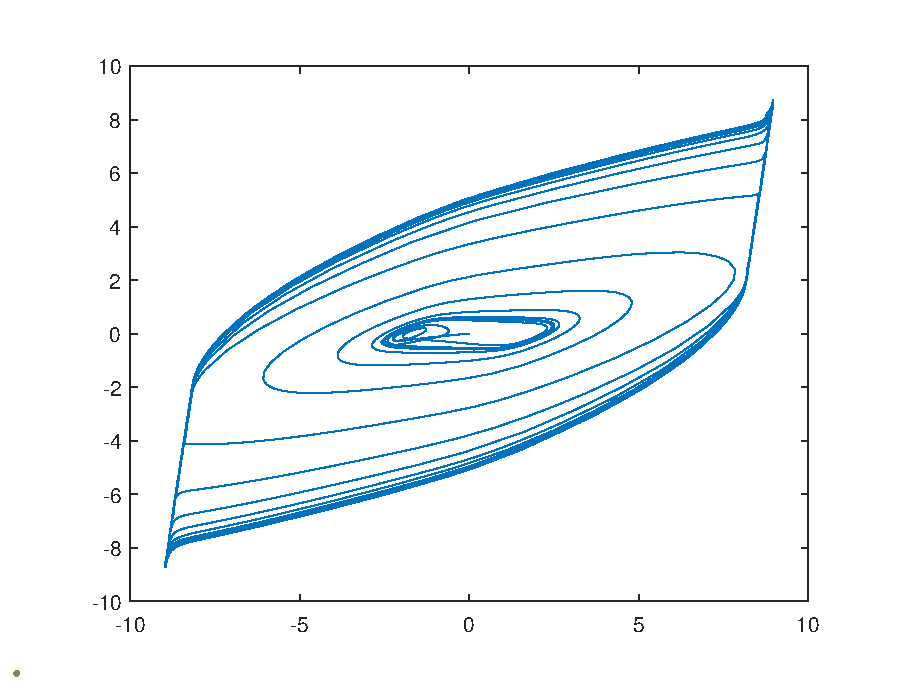
\includegraphics[width=.3\columnwidth]{R=1540,IL=0,VC2=0.01,VC2=-0.02.eps}
    }
    \subfigure[$V_{C2}=-0.01\mathrm{V}$]{
        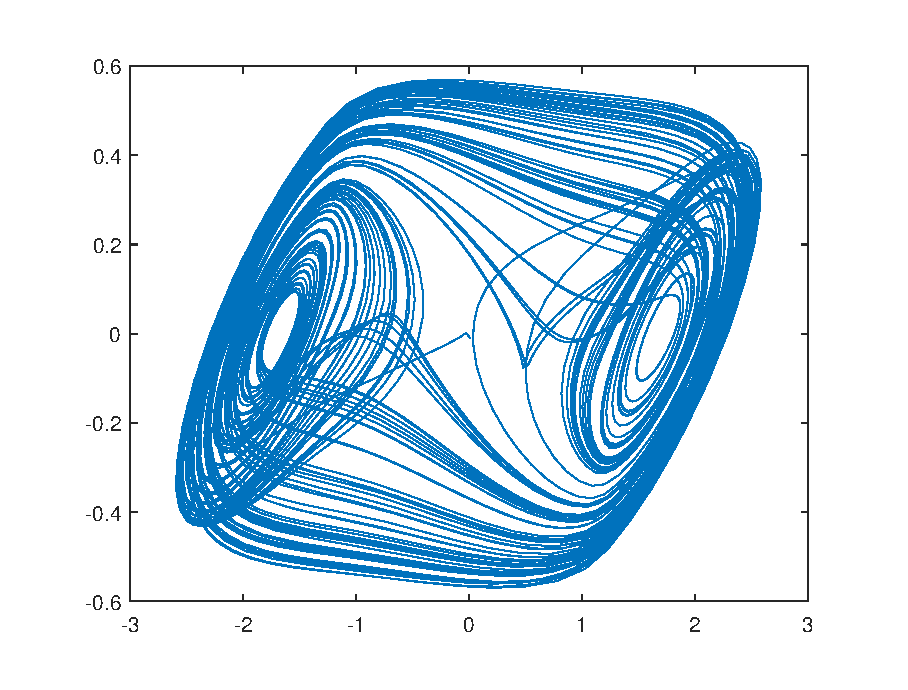
\includegraphics[width=.3\columnwidth]{R=1540,IL=0,VC2=0.01,VC2=-0.01.eps}
    }
    \subfigure[$V_{C2}=0.00\mathrm{V}$]{
        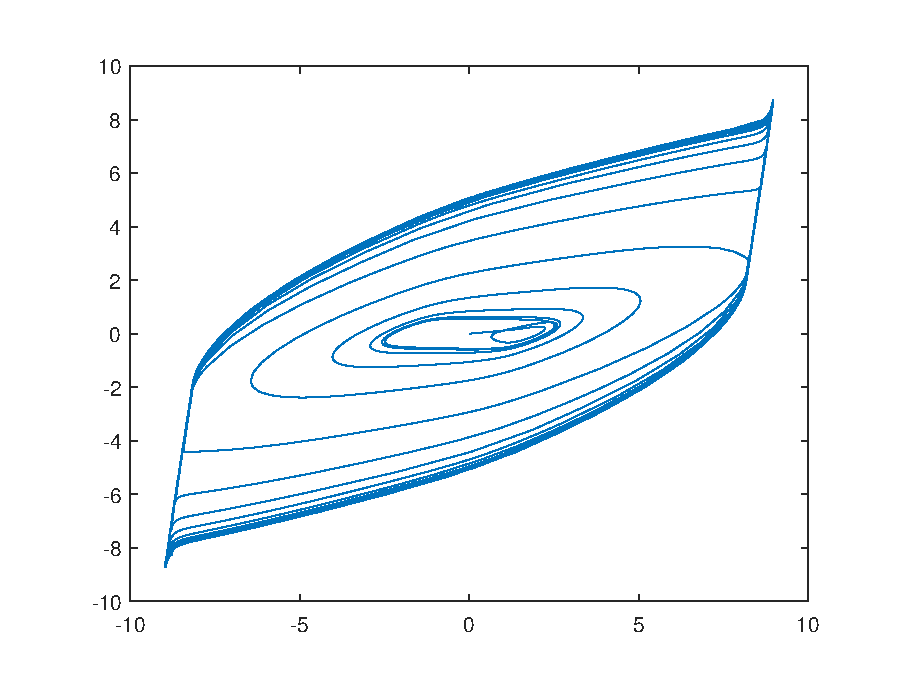
\includegraphics[width=.3\columnwidth]{R=1540,IL=0,VC2=0.01,VC2=0.eps}
    }
    \subfigure[$V_{C2}=0.01\mathrm{V}$]{
        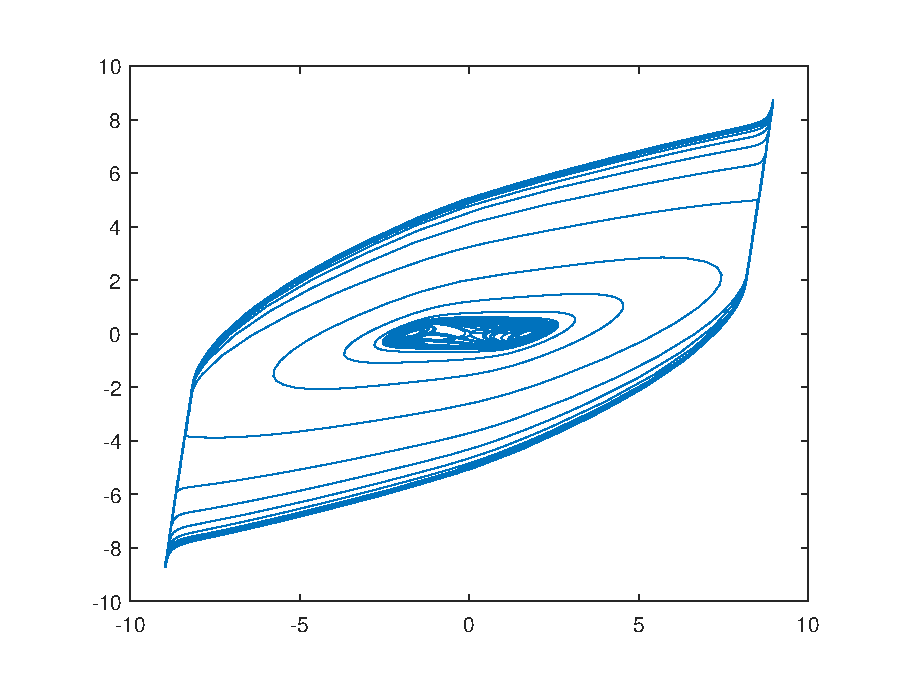
\includegraphics[width=.3\columnwidth]{R=1540,IL=0,VC2=0.01,VC2=0.01.eps}
    }
    \subfigure[$V_{C2}=0.02\mathrm{V}$]{
        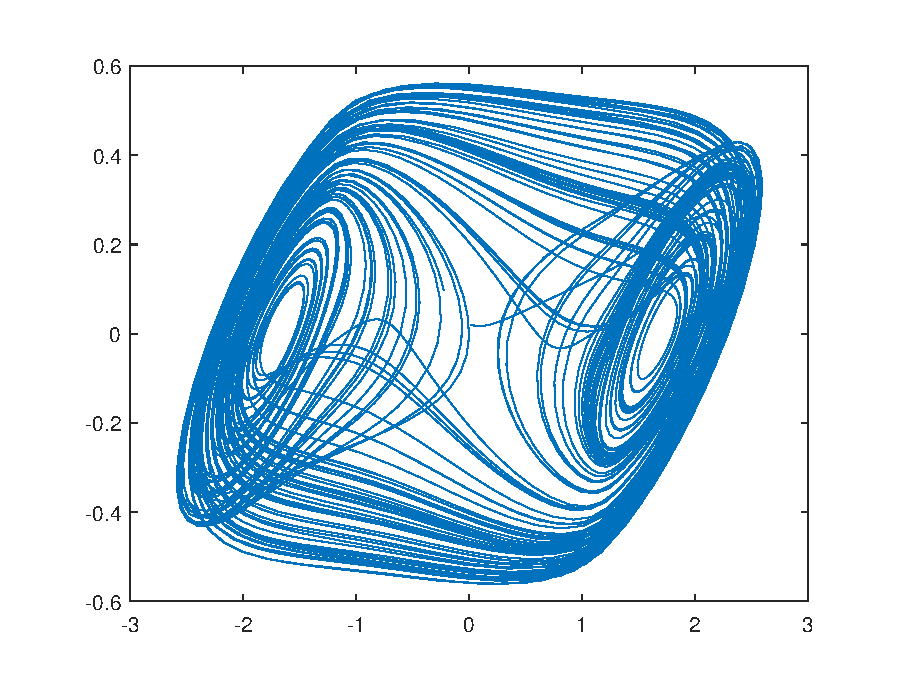
\includegraphics[width=.3\columnwidth]{R=1540,IL=0,VC2=0.01,VC2=0.02.eps}
    }
    \subfigure[$V_{C2}=0.03\mathrm{V}$]{
        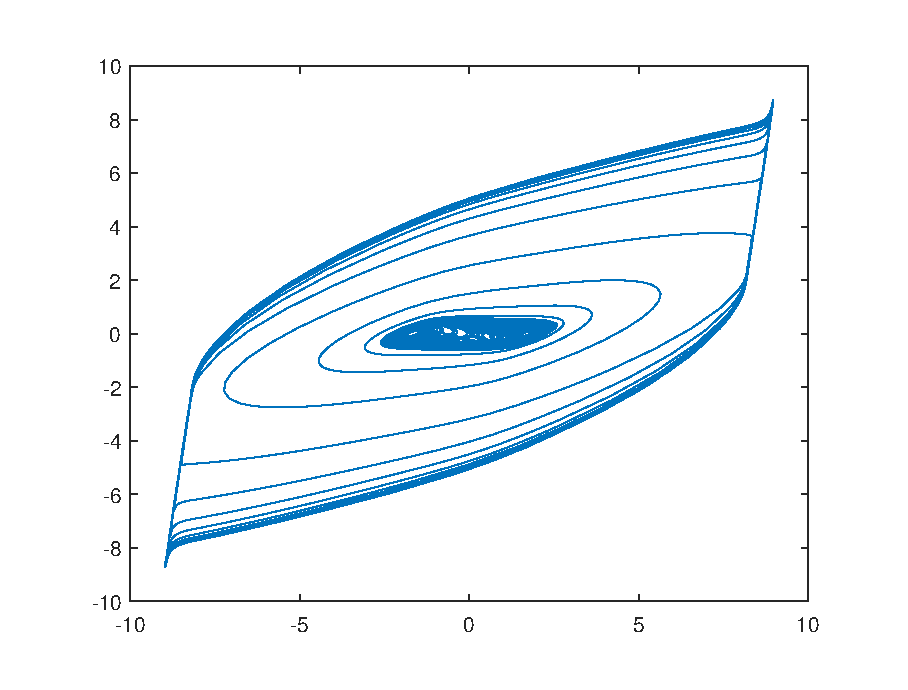
\includegraphics[width=.3\columnwidth]{R=1540,IL=0,VC2=0.01,VC2=0.03.eps}
    }
    \caption{设定可变电阻阻值$R=1540\mathrm{\Omega}$,初始条件$I_L(t=0)=0$,$V_{C1}(t=0)=0.01$,微调初始条件$V_{C2}(t=0)$得到的,以$V_{C1}$为横轴,以$V_{C2}$为纵轴的李萨如图}
    \label{vary-VC2}
\end{figure}

由图中,我们发现初始条件的微小改变就可以引起电路演化路径完全不同,这是混沌现象的典型体现.

\end{document}